%----------------------------------------------------------------------------------------
%	Metropolia Thesis LaTeX Template
%----------------------------------------------------------------------------------------
% License:
% This work is licensed under the Creative Commons Attribution 4.0 International License. 
% To view a copy of this license, visit http://creativecommons.org/licenses/by/4.0/.
%
% However, this license apply to this template. As a template, it is supposed to be 
% modified for your own needs (with your thesis content). For this reason, if you use 
% this project as a template and not specifically distribute it as part of a another 
% package/program, we grant the extra permission to freely copy and modify these files as 
% you see fit and even to delete this copyright notice. 
% In short, you are free to publish your thesis under whatever license you wish, even 
% keep the all rights reserved to you.
%
% Authors:
% Panu Leppäniemi, Patrik Luoto and Patrick Ausderau
%
% Credits:
% Panu Leppäniemi: abstract, def, cleaning,...
% Patrik Luoto: title page, abstract in Finnish, abbreviation, math,...
% Patrick Ausderau: initial version, style, table of content, bibliography, figure, 
%                   appendix, table, source code listing...
%
% Please:
% If you find mistakes, improve this template and alike, please contribute by sharing 
% your improvements and/or send us your feedback there: 
% https://github.com/panunu/metropolia-thesis-latex
% And of course, if you improve it, add yourself as an author.
%
% Compiler:
% Use XeLaTeX as a compiler.
 
%----------------------------------------------------------------------------------------
%	THESIS INFO
%----------------------------------------------------------------------------------------

% All general information (main language, title, author (you), degree programme, major 
% option, etc.)
% Edit the file chapters/0info.tex to change these information
% Global information (title of your thesis, your name, degree programme, major, etc.) 

\def\thesislang{finnish} %change this depending on the main language of the thesis. 
% "english" is the only other supported language currently. If someone has the swedish, please contribute!

\def\secondlang{english} %if the main language is Finnish (or Swedish), you must have 2 abstracts (one in Finnish (or Swedish) and one in English)
%If the main language is English and that you are native Finnish (or Swedish) speaker, you must have also abstract in your native language on top of the English one.

\author{Name} %your first name and last name
\def\thesis{Thesis}%keep the half based on the main thesis language
%was Opinnäytetyö

\def\alaotsikko{Subtitle} %if you don't have subtitle, empty {} it (but don't delete that line)

%Finnish section, for title/abstract
\def\otsikko{Opinnäytetyön otsikko}
\def\tutkinto{Tutkinto (esim. Insinööri (AMK))} % change to your needs, e.g. "YAMK", etc.
\def\kohjelma{Koulutusohjelma (esim. Tieto\textendash ja viestintätekniikka)}
\def\suuntautumis{Ammatillinen pääaine (esim. Mobile Solutions)}
\def\ohjaajat{
Titteli Etunimi Sukunimi\newline
Titteli Etunimi Sukunimi
}
\def\avainsanat{avainsanat}
\def\pvm{\specialdate\today}

%English section, for title/abstract
\title{Your title here}
\def\metropoliadegree {Bachelor of Engineering} % change to your needs, e.g. "master", etc.
\def\metropoliadegreeprogramme {your degree programme (e.g. Information Technology)}
\def\metropoliaspecialisation {your major option (e.g. Mobile Solutions)}
\def\metropoliainstructors {
First name Last name, Title (for example: Project Manager)\newline
First name Last name, Title (for example: Principal Lecturer)
}
\def\metropoliakeywords {Keywords}
\date{\longmonth\today}




%----------------------------------------------------------------------------------------
%	GLOBAL STYLES
%----------------------------------------------------------------------------------------

% If you need extra package, etc. modify the style/style.tex file.
% If you are using Windows OS, you will need to change default font to Arial in that 
% style/style.tex file (or install Liberation Sans font to your system).
% If you are using MacOS or linux, make sure you have Liberation Sans font installed.
% Global style. Normally should not be edited. 
% If you use windows OS, eventually change \setmainfont to Arial
% Check around commit https://github.com/panunu/metropolia-thesis-latex/commit/a0c15ac77bab1a52c59c517a18080938e57bf5ef
% to see how the font files were manually added (after downloading them: https://pagure.io/liberation-fonts/ )

\documentclass[11pt,a4paper,oneside,article]{memoir}
\usepackage[\secondlang,\thesislang]{babel}% finnish english swedish
\usepackage{iflang}
\usepackage{amsmath}
\usepackage{amsfonts}
\usepackage{amssymb}
\usepackage{fontspec}
\usepackage{tocloft}
\usepackage{titlesec}
\usepackage[hyphens]{url}
\usepackage{mathtools}
\usepackage{wallpaper}
\usepackage{datetime}
\usepackage[bookmarksdepth=subsection]{hyperref} % for automagic pdf links for toc, refs, etc.
\usepackage[amssymb]{SIunits}
\usepackage[version=3]{mhchem}
\usepackage{pgfplots} %simple plots etc
\usepackage{pgfplotstable}
\usepackage{tikz} % mindmaps, flowcharts, piecharts, examples at http://www.texample.net/tikz/examples/
\usetikzlibrary{shapes.geometric, arrows}


\renewcommand{\dateseparator}{.}
%condition for adding or not space in TOC
\usepackage{etoolbox}
%for compact list
\usepackage{enumitem}
%for block comment
\usepackage{verbatim}
%for "easier" references
\usepackage{varioref}
%forcing single line spacing in bibliography
\DisemulatePackage{setspace}
\usepackage{setspace}
%including figure (image)
\usepackage{graphicx}
\usepackage{caption}
\usepackage{subcaption}
%change the numbering for figure
\usepackage{chngcntr}
%strike trough
\usepackage{ulem}
%euro symbol
\usepackage{eurosym}
%try to count
\usepackage{totcount}
%insert source code
%\usepackage{listings}
%require -8bit -shell-escape in the xelatex compile command
\usepackage[newfloat]{minted}
\setminted{tabsize=2,linenos,breaklines,breaksymbolleft={\quad},baselinestretch=1}
\setmintedinline{breaklines}
\usepackage[justification=justified,singlelinecheck=false]{caption}
\usepackage{color}
%force the width of a table instead of column
\usepackage{tabularx}
\usepackage{booktabs} %why not booktabs? :3
% Abbreviations, acronym and glossary
\usepackage[acronym,nonumberlist,section]{glossaries}%xindy,%toc, ,nomain

\usepackage{float} % For forced figure location with modifier H (\begin{figure}[H])
\usepackage{cite} % Make citations to match Metropolia thesis guide

% change font of links in bibliography to same as other text
\usepackage{url}
\urlstyle{same}

% change punctuation of multiple cites to semicolon instead of comma: [1; 2; 3]
\renewcommand\citepunct{; }

% citep-macro for reference with period inside square brackets [1.]
\newcommand{\citep}[1]{
 \renewcommand\citeright{.]}
 \cite{#1}
 \renewcommand\citeright{]}
}

%set date format to D.M.YYYY
\newdateformat{specialdate}{\THEDAY.\THEMONTH.\THEYEAR}
%set date format to D Month YYYY
\newdateformat{longmonth}{\THEDAY~\monthname[\THEMONTH] \THEYEAR}

\newcommand\tn[1]{\textnormal{#1}} %use \tn instead of \textnormal
\newcommand\reaction[1]{\begin{equation}\ce{#1}\end{equation}} %\reaction{} for chemical reactions

%NORMAL TEXT
%all text, title, etc. in the same font: Arial
%NOTE: fontname is case-sensitive
\setmainfont{Arial}
%line space
\linespread{1.5}
\AtBeginEnvironment{tabular}{\singlespacing}
%\doublespacing
%margin
\usepackage[top=2.5cm, bottom=3cm, left=4cm, right=2cm, nofoot]{geometry}
\setlength{\parindent}{0pt} %first line of paragraph not indented
\setlength{\parskip}{16.5pt} %one empty line to separate paragraph
%list with small line space separation
\tightlists

%IMAGE - FIGURE
%the figures should be placed in the "illustration" folder
\graphicspath{{illustration/}}
%figure number without chapter (1.1, 1.2, 2.1) to (1, 2, 3)
\counterwithout{figure}{chapter}
%border around images
\setlength\fboxsep{0pt}
\setlength\fboxrule{0.5pt}
%caption font size
\captionnamefont{\small}
\captiontitlefont{\small}
%space after figure caption (and other float elements)
\setlength{\belowcaptionskip}{-7pt}

%TABLE
\counterwithout{table}{chapter}

%SOURCE CODE
\newenvironment{code}{\captionsetup{type=listing}}{}
\IfLanguageName {finnish} {\SetupFloatingEnvironment{listing}{name=Listing}} {}
%\counterwithout{lstlisting}{chapter}
%moved after begin document, otherwise does not compile

%% set this format as the default for lstlisting
%\DeclareCaptionFormat{empty}{}
%\captionsetup[lstlisting]{format=empty}

%TOC
%change toc title
\IfLanguageName {finnish} {\addto{\captionsfinnish}{\renewcommand*{\contentsname}{Contents}}} {}
%remove dots
\renewcommand*{\cftdotsep}{\cftnodots}
%chapter title and page number not in bold
\renewcommand{\cftchapterfont}{}
\renewcommand{\cftchapterpagefont}{}
%sub section in toc
\setcounter{tocdepth}{2}
%subsection numbered
\setcounter{secnumdepth}{2}
\renewcommand{\tocheadstart}{\vspace*{-15pt}}
\renewcommand{\printtoctitle}[1]{\fontsize{13pt}{13pt}\bfseries #1}
\renewcommand{\aftertoctitle}{\vspace*{-22pt}\afterchaptertitle}
%spacing afer a chapter in toc
\preto\section{%
  \ifnum\value{section}=0\addtocontents{toc}{\vskip11pt}\fi
}
%spacing afer a section in toc
\renewcommand{\cftsectionaftersnumb}{\vspace*{-3pt}}
%spacing afer a subsection in toc
\renewcommand{\cftsubsectionaftersnumb}{\vspace*{-1pt}}
%appendix in toc with "Appendix " + num
\IfLanguageName {finnish} {
  \renewcommand*{\cftappendixname}{Appendix\space}
  \renewcommand{\appendixtocname}{Appendices}
}{\renewcommand*{\cftappendixname}{Appendix\space}}
%appendix header
\IfLanguageName {finnish} {\def\appname{Appendix\space}}{\def\appname{Appendix\space}}

%TITLES
%chapter title
%\clearforchapter{\clearpage}
\titleformat{\chapter}
{\fontsize{13pt}{13pt}\bfseries\linespread{1}}%\clearpage
{\thechapter}{.5cm}{}
\titlespacing*{\chapter}{0pt}{.32cm}{9pt}
\titleformat{\section}
{\fontsize{12pt}{12pt}\linespread{1}}
{\thesection}{.5cm}{}
\titlespacing*{\section}{0pt}{14pt}{6pt}
\titleformat{\subsection}
{\fontsize{12pt}{12pt}\linespread{1}}
{\thesubsection}{.5cm}{}
\titlespacing*{\subsection}{0pt}{14pt}{6pt}


%QUOTE
\renewenvironment{quote}
  {\list{}{\rightmargin=0pt\leftmargin=1cm\topsep=-10pt}%
  \item\relax\fontsize{10pt}{10pt}\singlespacing}
  {\endlist}

%BIBLIOGRAPHY
%bibliography title to be "references"
%IF THE TITLE DON'T GET RENAMED PROPERLY, move that line after the \begin{document}
\IfLanguageName {finnish} {\addto{\captionsfinnish}{\renewcommand*{\bibname}{References}}} {\renewcommand\bibname{References}}
\makeatletter %reference list option change
\renewcommand\@biblabel[1]{#1\hspace{1cm}} %from [1] to 1 with 1cm gap
\makeatother %
\setlength{\bibitemsep}{11pt}

%count the appendices (since the chapter counter is reset after \appendix).
%! require to complie 2 times
\regtotcounter{chapter}


\makepagestyle{tiivis}
\makeevenhead{tiivis}{}{}{Tiivistelmä}
\makeoddhead{tiivis}{}{}{Tiivistelmä}

\makepagestyle{abstract}
\makeevenhead{abstract}{}{}{Abstract}
\makeoddhead{abstract}{}{}{Abstract}



% Normally, you do not need to modify the title style. It's content comes from the 
% chapters/0info.tex file.
% TITLE PAGE
% Normally, you should not edit this file.

\makeatletter
\renewcommand{\maketitle}{
\thispagestyle{empty}
\ThisCenterWallPaper{1}{viiva}
%
\vspace*{8.5cm}
\tn{\LARGE\@author\\[22pt]\Huge\IfLanguageName {finnish}{\otsikko}{\@title}\\[22pt]\LARGE\alaotsikko\\[1.75cm]}

\parbox{.7\linewidth}{
\IfLanguageName {finnish}{
  Helsinki Metropolia University of Applied Sciences\\
  \tutkinto \\
  \kohjelma \\
  \thesis\\
  \pvm
} {
  Helsinki Metropolia University of Applied Sciences\\
  \metropoliadegree \\
  \metropoliadegreeprogramme \\
  \thesis\\
  \IfLanguageName {finnish}{\pvm}{\@date} % D.M.YYYY date format for Finnish. D Month YYYY for English
}
}
\ThisLRCornerWallPaper{1}{metropolia}
%
\clearpage
}
\makeatother



%----------------------------------------------------------------------------------------
%	ABBREVIATION AND GLOSSARY
%----------------------------------------------------------------------------------------

% Add/edit all your acronyms, abbreviations, glossary entries, etc. definitions in 
% chapters/0abbr.tex file.
% You can have as many as you wish. Only the ones you use in your text (inserted with 
% \gls{} command) will print in the Glossary/Lyhenteet.
% Generate the glossary

\makeglossaries

% Acronyms, abbreviations, etc. 

\newacronym{scv}{CSV}{Comma Separated Values file}
\newacronym{pp}{PP}{Polypropylene- plastic}
\newacronym{efd}{EFD}{Experimental Fluid Dynamics}
\newacronym{cfd}{CFD}{Computational Fluid Dynamics}
\newacronym{ltd}{SansOx Ltd.}{SansOx Limited}
\newacronym{dn}{DN}{Diameter Nominal}
\newacronym{cad}{CAD}{Computer-Aided Design}


% Glossary entries

\newglossaryentry{cavit}{
	name={cavitation}, 
	description={the formation of vapour cavities in a liquid, small liquid-free zones ("bubbles" or "voids")}
}
\newglossaryentry{viscos}{
	name={viscosity}, 
	description={resistance of a fluid (liquid or gas) to a change in shape, or movement of neighbouring portions relative to one another.}
}





%----------------------------------------------------------------------------------------
%	DOCUMENT STARTS HERE...
%----------------------------------------------------------------------------------------

\begin{document}
\counterwithout{listing}{chapter}

%----------------------------------------------------------------------------------------
%	TITLE PAGE
%----------------------------------------------------------------------------------------

\input{style/title_headers.tex}
\maketitle
\newpage
%all abstract, table of content and glossary will get the metropolia logo at bottom
\LRCornerWallPaper{1}{footer}

%----------------------------------------------------------------------------------------
%	ABSTRACT / Tiivistelmä
%----------------------------------------------------------------------------------------

% If you are international student writing in English, remove the Finnish abstract.
% If you are Finnish citizen, you must have 2 abstracts, one in Finnish (or Swedish 
% depending on your mother tongue) and one in English regardless of the main language of 
% your thesis.
% \input{chapters/0abstract_fi.tex}
% Abstract in English
%Most probably, you only need to change the text of the abstract. Everything else comes from chapter/0info.tex
%If you do not have any appendix, you may delete \total{chapter} and replace with 0

\pagestyle{abstract}
\begin{otherlanguage}{english}
{\renewcommand{\arraystretch}{2}%
\begin{tabular}{ | p{4,7cm} | p{10,3cm} |}
  \hline
  Author(s) \newline
  Title \newline\newline 
  Number of Pages \newline
  Date
  & 
  \makeatletter
  \@author \newline
  \@title \newline\newline
  \pageref*{LastPage} pages + \total{chapter} appendices \newline %! if no appendices, risk to count total of chapter :D
  \IfLanguageName {finnish} {\foreignlanguage{english}{\longdate\@date}} {\@date}
  \makeatother
  \\ \hline
  Degree & \metropoliadegree
  \\ \hline
  Degree Programme & \metropoliadegreeprogramme
  \\ \hline
  Professional Major & \metropoliaspecialisation
  \\ \hline
  Instructor(s) & \metropoliainstructors
  \\ \hline
  \multicolumn{2}{|p{15cm}|}{\vspace{-22pt}
 Reducing energy dissipation inside a tube in fluid process engineering is one of the key factors to improve the efficiency of an industrial process. The purpose of this project is to demonstrate the ability to reduce fluid energy dissipation by utilizing a half elliptical blade wing named Voxer from \gls{ltd} inside a pipeline. The project was carried out by performing comparative testing on replication models of pipeline section belonging to water cooling system at Keravan Energy's biomass power plant. The Voxer inherits features from static mixer to create vortex current and has innovative characteristics to act as a cost-effective add-on solution for existing pipeline systems. 
 \newline
  
Fluid Flow experimentation on Voxer by measuring pressure drop shows that with the correct position of Voxer in the system, raising of vortex flow reduces pressure drop, which is proportional with decreasing energy losses in the fluid.
  } \\[14cm] \hline
  Keywords & \metropoliakeywords
  \\ \hline
\end{tabular}
}
\end{otherlanguage}
\clearpage



%----------------------------------------------------------------------------------------
%	License? Acknowledgement?
%----------------------------------------------------------------------------------------

% Uncomment next line and edit chapters/0license.tex if you want license in your thesis.
%\input{chapters/0license.tex}

% Uncomment next line and edit chapters/0acknowledgement.tex if you want acknowledgements.
\input{chapters/0acknowledgement.tex}

%----------------------------------------------------------------------------------------
%	TABLE OF CONTENTS
%----------------------------------------------------------------------------------------

\input{style/toc.tex}

%list of figure, tables would come here if relevant?

%----------------------------------------------------------------------------------------
%	Lyhenteet / Abbreviation
%----------------------------------------------------------------------------------------

% If you don't use abbreviations/glossary, remove the following line.
% Abbreviation and Glossary
% Normally, you don't have to modify this file. Your abbreviations, etc. goes in 
% ../chapters/0abbr.tex file.

\begin{singlespacing}

% \gsladdall would add all terms even if not used in your text.
%\glsaddall

{
	\titleformat{\section}
	{\fontsize{13pt}{13pt}\bfseries\linespread{1}}
	{\thesection}{.5cm}{}
	%Adapt labelwidth (sorry for the ugly hack)
	\setlist[description]{leftmargin=!, labelwidth=4em}
	\IfLanguageName {finnish} {
		\printacronyms[title=Abbreviations]
	}{
		\printacronyms[title=Abbreviations]
	}
	\setlist[description]{leftmargin=!, labelwidth=7em}
	\printglossary 
	\setlist[description]{style=standard} % reset settings back to default
}
\end{singlespacing}

\clearpage


%----------------------------------------------------------------------------------------
%	CONTENT
%----------------------------------------------------------------------------------------

\input{style/content.tex}%reset page number to 1, no more logo footer, etc.

% Thesis content if you strictly follow the "Final Year Project guide". Of course, you 
% can adapt to your specific needs (add more chapter, rename them, etc.).
% Introduction

\chapter{Introduction}

Minimizing fluid energy losses is one of important missions in hydraulic engineering and chemical engineering to improve the overall efficiency of the system. The flow resistance in pipe is caused by various reasons, such as \gls{viscos}, pipe roughness or change of velocity.\newline
The new product from \gls{ltd} is an economic solution to this problem. The product is called Voxer, which consists of a Voxer wing to be inserted into a tube . The wing creates vortex flow that reduces turbulence and flow loss in the tube. Voxer can be installed in various places allocated accordingly in a whole pipeline. 

The objectives of this thesis is to present Voxer's function in reducing energy consumption in pipe and to examine the affect of different Voxer wing's combinations. The thesis was also carried out to analyze the hydraulic phenomenon and determine the Voxer's performance when introducing to the market.

The experiments were conducted in Keravan Bio-power plant of Keravan Energy Limited. Keravan Energy Ltd. is a state owned company in Kerava and Sipoo municipality. They produce electricity and district heating to not only serve their own municipality but also to sell electricity to the whole Finland. The object of this study is the water cooling piping system of the power plant.\newline
SansOx Limited is the commissioner of this project. \gls{ltd} focuses on researching, developing and marketing fresh innovation solutions for clean water market worldwide. Their goal is to advanced products in order to provide the optimal sustainable solutions for customers' needs in water treatment, process wastewater treatment, fish farming and agriculture. By executing this study, we will contribute to a completed theory profile of Voxer with quantitative research regarding to hydraulic and geometrical parameters of industrial piping system. 

In this thesis, we will demonstrate the experimental fluid dynamics setup and analysis on Voxer under laboratory condition and realistic condition in the power plant. Also, the limitation and possible further study will be discussed. 

\clearpage %force the next chapter to start on a new page. Keep that as the last line of your chapter!

% uncomment what you need.
%% Project Specifications

\chapter{Project Specifications}

Check Final Year Project Guide for the content of Project Specifications chapter.

\clearpage %force the next chapter to start on a new page. Keep that as the last line of your chapter!

%% Theoretical background

\chapter{Theoretical background}

Check Final Year Project Guide for the content of Theoretical background chapter.

\clearpage %force the next chapter to start on a new page. Keep that as the last line of your chapter!

%% Project Specifications

\chapter{Project Specifications}

Check Final Year Project Guide for the content of Project Specifications chapter.

\clearpage %force the next chapter to start on a new page. Keep that as the last line of your chapter!

%% Material and Methods

\chapter{Methodology}
Fluid Flow Experiment was attempted  
\section{Measurement parameters}
\section{Instruments and equipments}

\clearpage %force the next chapter to start on a new page. Keep that as the last line of your chapter!

%% Experiments

\chapter{Experimentation}
In this chapter, we will go through the process, result and analysis of two experiments for Voxer's comparative testing in Keravan Energy's cooling system. The pressure meter used in both tests is Danfoss PFM 100 \cite{danfoss:web} which measures Kv factor, pressure and flow rate. All of equipments and components needed for operation are mentioned in appendix. The CAD models for pipeline and source code for analysis are also presented in appendix. Figure \vref{fig:orgpipe} shows the original cooling piping section in Keravan Energy. The pipeline includes these main components: one 5 meters of straight pipe, two 90$^{\circ}$ curves and rubber hoses. The pipe used in Keravan Energy is DN50.
\begin{figure}[h]
  \centering
  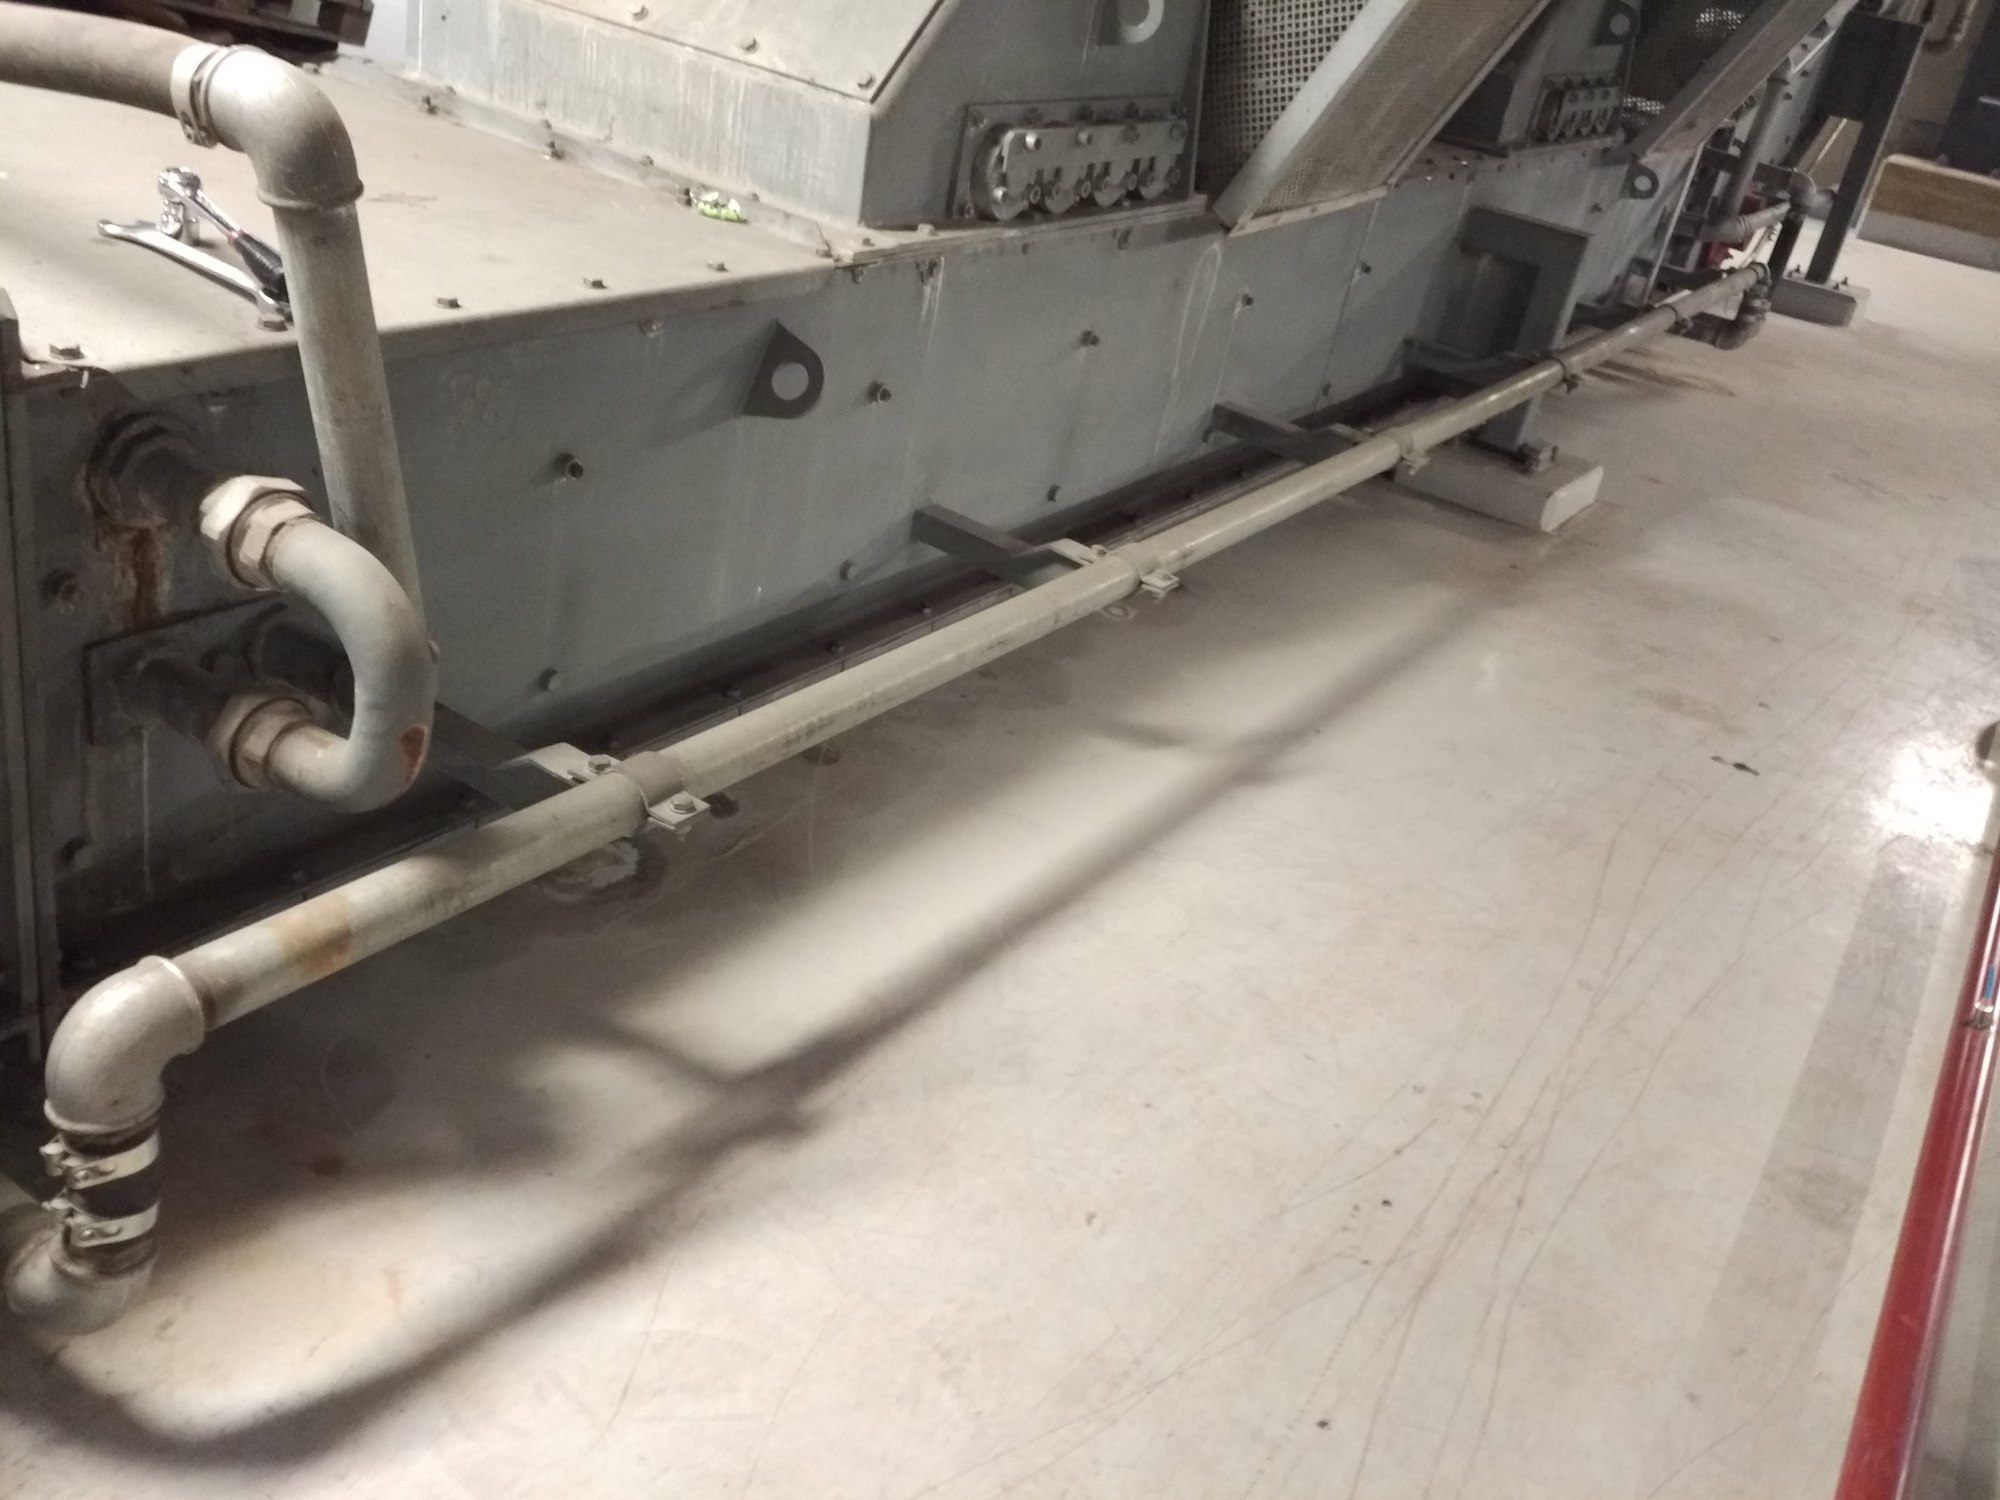
\includegraphics[width=8cm]{original_pipe}
  \caption{ Targeted piping system in Keravan Energy}
  \label{fig:orgpipe}
\end{figure}
\section{Laboratory experimentation}
It is essential to get a full understanding about the hydraulic system, product testing and objectives. In order to achieve this, it is advised to perform comparative measurements under laboratory condition first. In this setting, we will acquire more knowledge about factors which could affect to the system, proper techniques, required conditions and practices which needed to be applied to ensure the quality of measurement. Moreover, the data acquired would be more stable under controlled setting.
\subsection{Experiment's design}
The main goal of this laboratory experimentation is setting up the closest replication of cooling piping section with PP material and determining which Voxer combination is the best for the real test in Keravan Energy. Apart from that, there are some other learning points in this test also; for example: understanding the structure of the targeted pipeline, learning about Voxer and how to assemble it into the system, insights from impacts of different setting conditions to the result of measurements.
\begin{figure}[h]
  \centering
  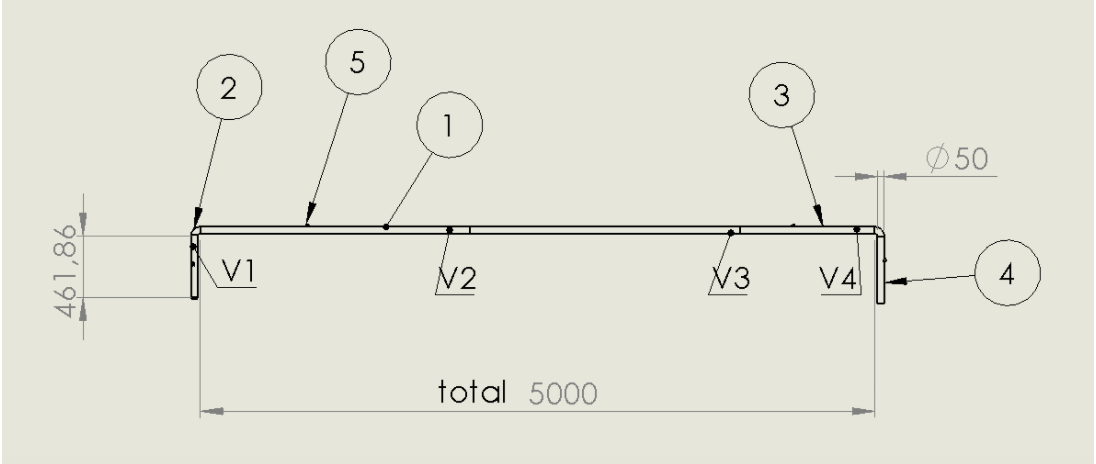
\includegraphics[width=8cm]{cadlab}
  \caption{ Basic pipe layout and positions of measuring points and Voxer wings \newline 1) Straight pipes 2 m; 2) 90$^{\circ}$ curves; 3) Straight pipe 1 m; 4) Straight pipe 0.5 m; 5) Plane connectors for measuring points}
  \label{fig:cadlab}
\end{figure}
Figure \vref{fig:cadlab} illustrated the basic setting of the pipelines. There are 4 measuring points which associates with plane connectors. The reason for creating these connectors is to create flat surface for ensuring secured pressurization of measuring points. It also minimizes the interference of the measuring device to the pressure and flow in the system. Each Voxer is connected to the end of each straight pipe, except the last one. There are maximum 4 Voxers using in each of measurement. With this settings, the pipeline is divided into 3 sections as pipes in series where total pressure is the accumulation of pressure from each section of the whole pipeline. In this experiment, we named section A from point 1 to 2, section B from point 2 to 3 and section C from point 3 to 4. Section T indicates the whole pipe from point 1 to 4 as the beginning and the end of the system. 
Since pipes are connected in series, we have:
\begin{align}
\delta P_t&= P_a + P_b + P_c = P_ab + P_c \\
\delta P_t&= \tn{Total pressure change in pipeline} \\
P_a&= \tn{Pressure change in section A} \\
P_b&= \tn{Pressure change in section B} \\
P_c&= \tn{Pressure change in section C} \\
P_ab&= \tn{Pressure change in section A and B} \\
\end{align}
There are 2 types of Voxer which were used in the test : Voxer 40$^{\circ}$ DN40 and Voxer 30$^{\circ}$ DN40.  Different combinations of the amount of Voxer and types of Voxer were carried out to determine the behavior of flow in each section and find out the best combination. Table \ref{table:combi} lists out the combinations performed in this test. The pressure changes between section A, section A and B and total pipe were measured in every combination. Every measurement was repeated 10 times to ensure balanced values. During the test, the average temperature of water in vessel was measured also to consider its influence on fluid viscosity and surface tension. Measurement for empty pipe was performed as well. Inner diameter of the pipe was measured to have Voxer customized as a perfect fit inside the tube. The material of pipes is PP.
\begin{table}[h]
  \centering
  \caption{Voxer combinations in lab test.\newline (V1 : Voxer in pipe 1; V12: Voxers in pipe 1 and 2, etc)}
  \begin{tabular}{l*{6}{c}}
Type             & V0 & V1 & V12 & V123 & V1234 & V14 \\
\hline
None & X & - & - & - & - & -   \\
30 degree           & - & X & X & X &  X & X  \\
40 degree           & - & X & X & X &  X & X   \\
Mixed     & - & - & - & - & - & X   \\
\end{tabular}
  \label{table:combi}
\end{table}
\subsection{Setting of experiments}
\textbf{Main pipe} \newline
The pipeline test system was set like firgure \vref{fig:cadlab} in Metropolia’s laboratory.  Pipes were connected with others in series. The main straight horizontal pipe section is 5 meters long in total, which included two 2 meters of straight pipes and one 1 meter of straight pipe. Each side of main straight pipe was fitted with a 90$^{\circ}$ curve. There were two 0.5 meters of vertical pipe extensions at each side, acting as extended pipes for placing Voxer and measuring points. Two reducers were attached with these extended in order to accommodate the hose pump. Figure \vref{fig:wholepipe} demonstrates the completed setting of pipe.
\begin{figure}[h]
  \centering
  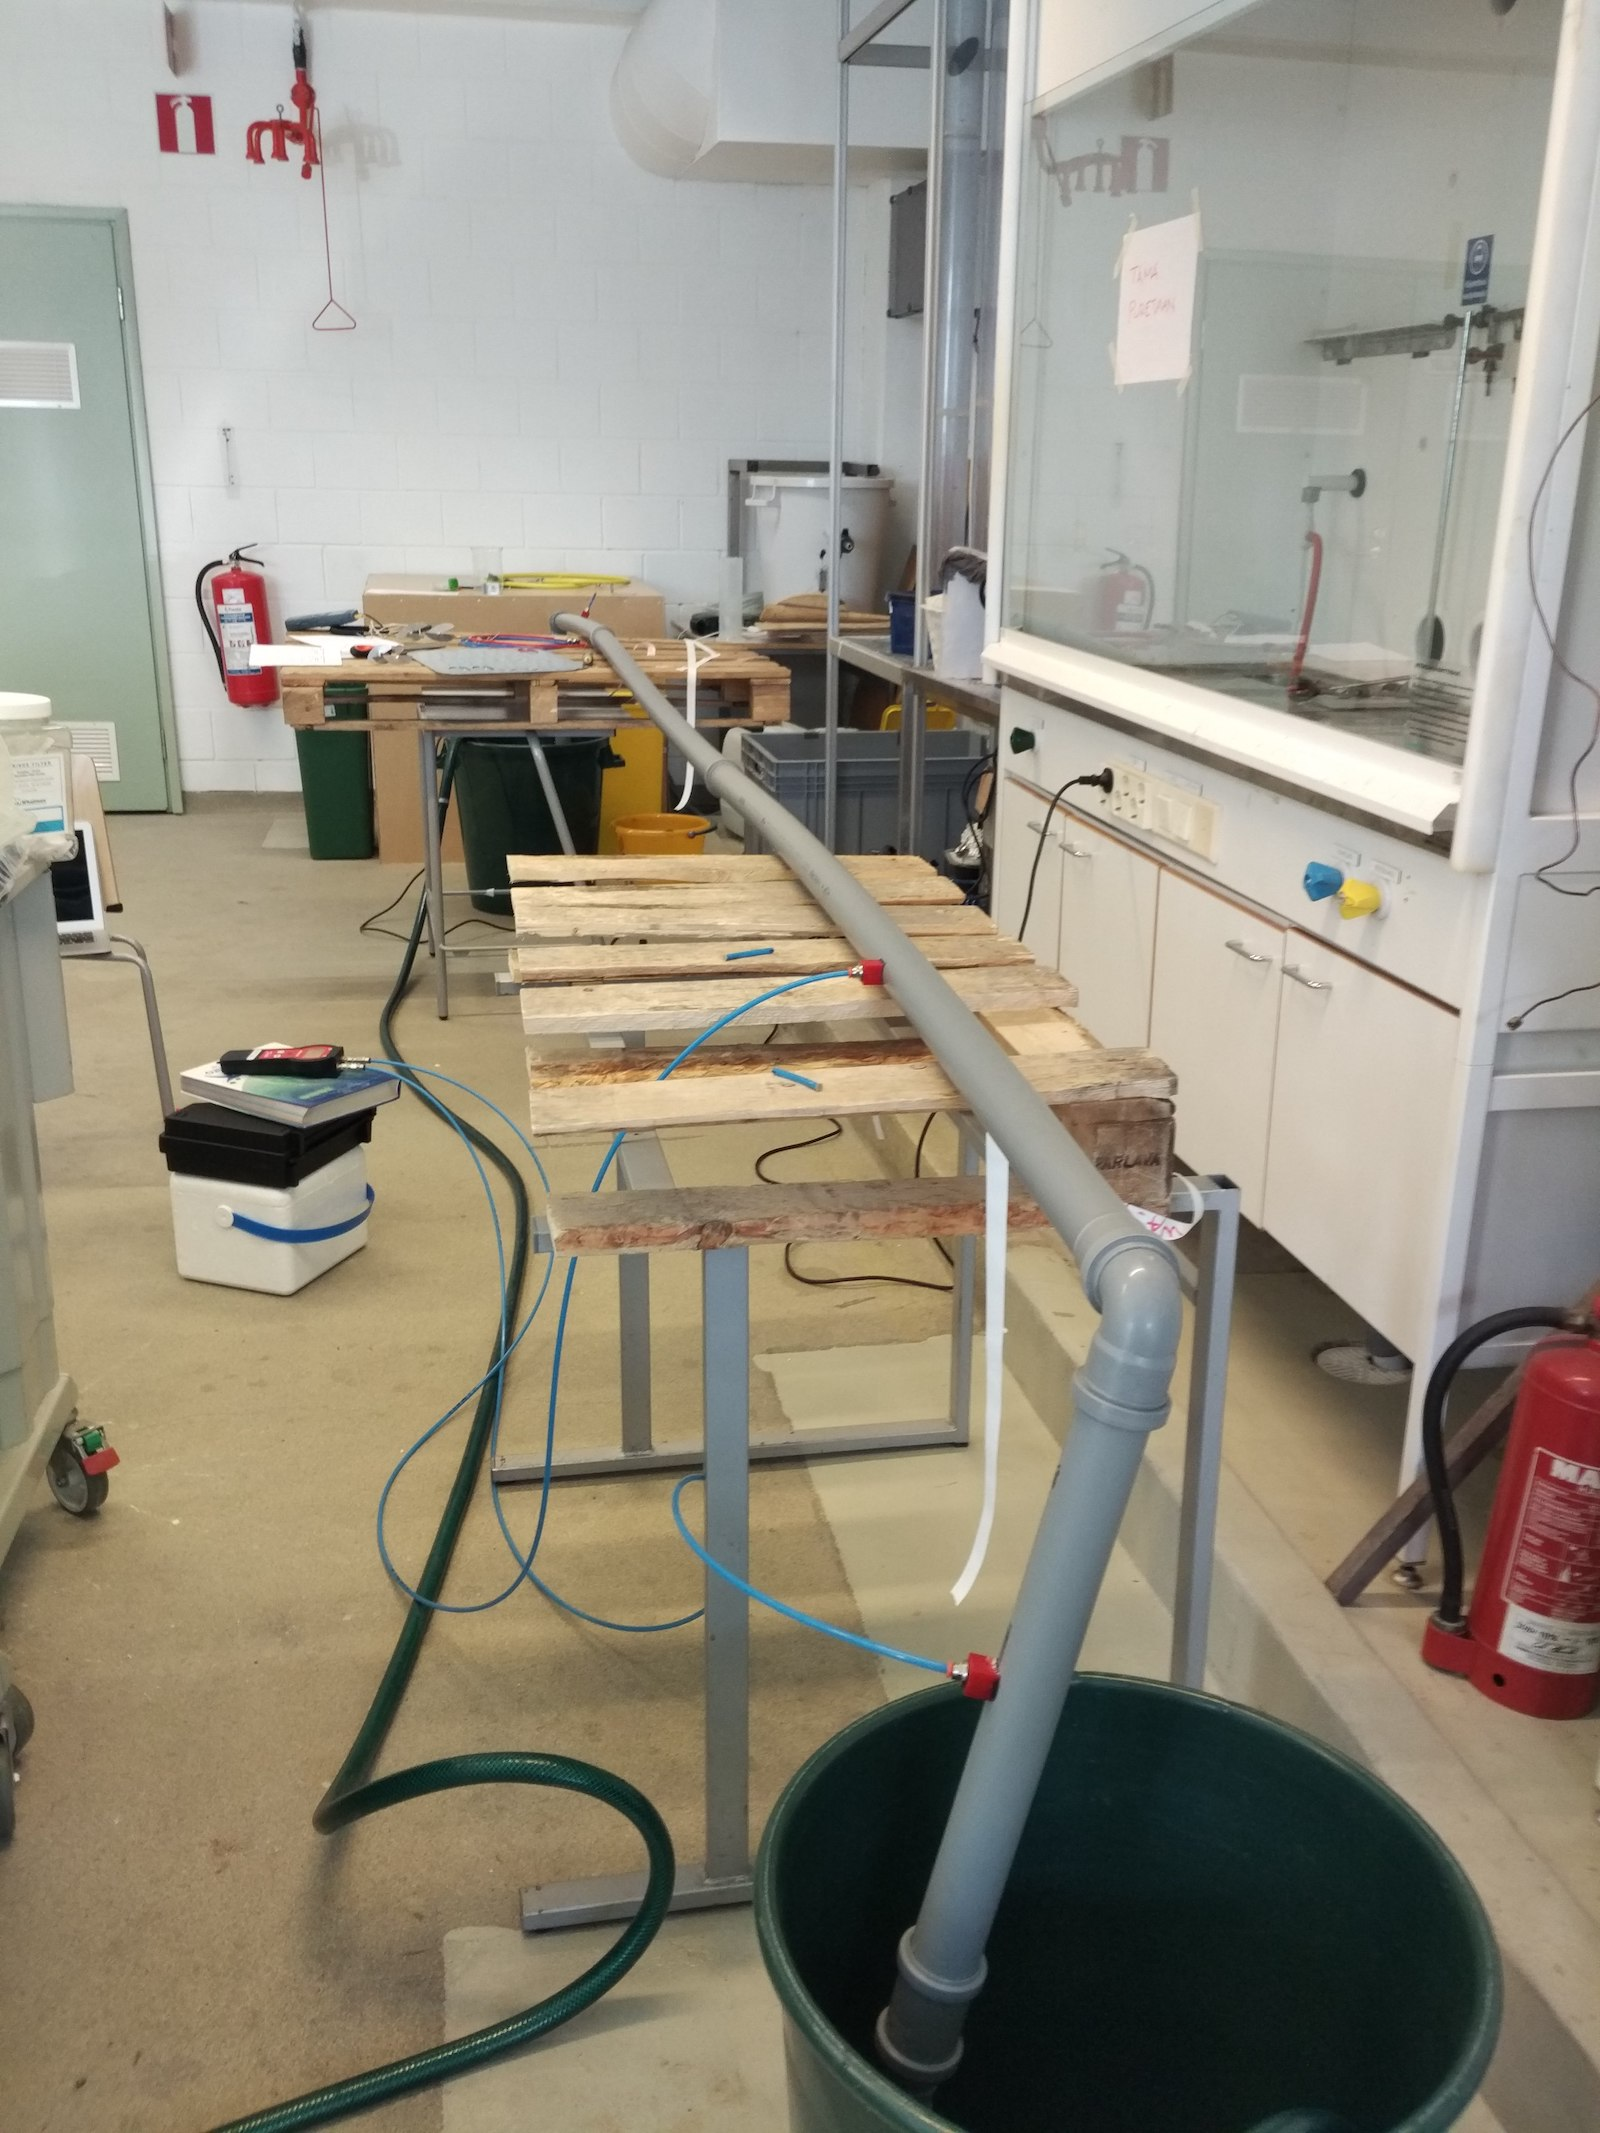
\includegraphics[width=8cm]{wholepipe}
  \caption{View of the whole test pipeline in Metropolia's lab }
  \label{fig:wholepipe}
\end{figure}

\textbf{Connectors, pump and vessels}\newline
Plastic connectors were 3-D printed. Pressure meter’s hoses were attached to the pipe by 4 plastic connectors glued above small holes on the pipe (see figure \vref{fig:connector}). Voxers were separated from metal sheet, bended and twisted following given instruction from SansOx Ltd. and inserted into different positions of the pipeline (see firgure \vref{fig:vox}). As mentioned before, the positions of Voxer were mainly at the end of each pipe. The system was set above the ground with 2 vessels at each side to keep the flow going with gravity, one as water reservoir and one for precaution leaking. A pump was positioned in water reservoir and connected with the starting pipe by hose. Water was delivered through the system and come back to the water reservoir. The ending pipe was submerged completely into water to balance static pressure in the system (see figure \vref{fig:subpipe}).

\begin{figure}[!htb]
   \begin{minipage}{0.48\textwidth}
     \centering
     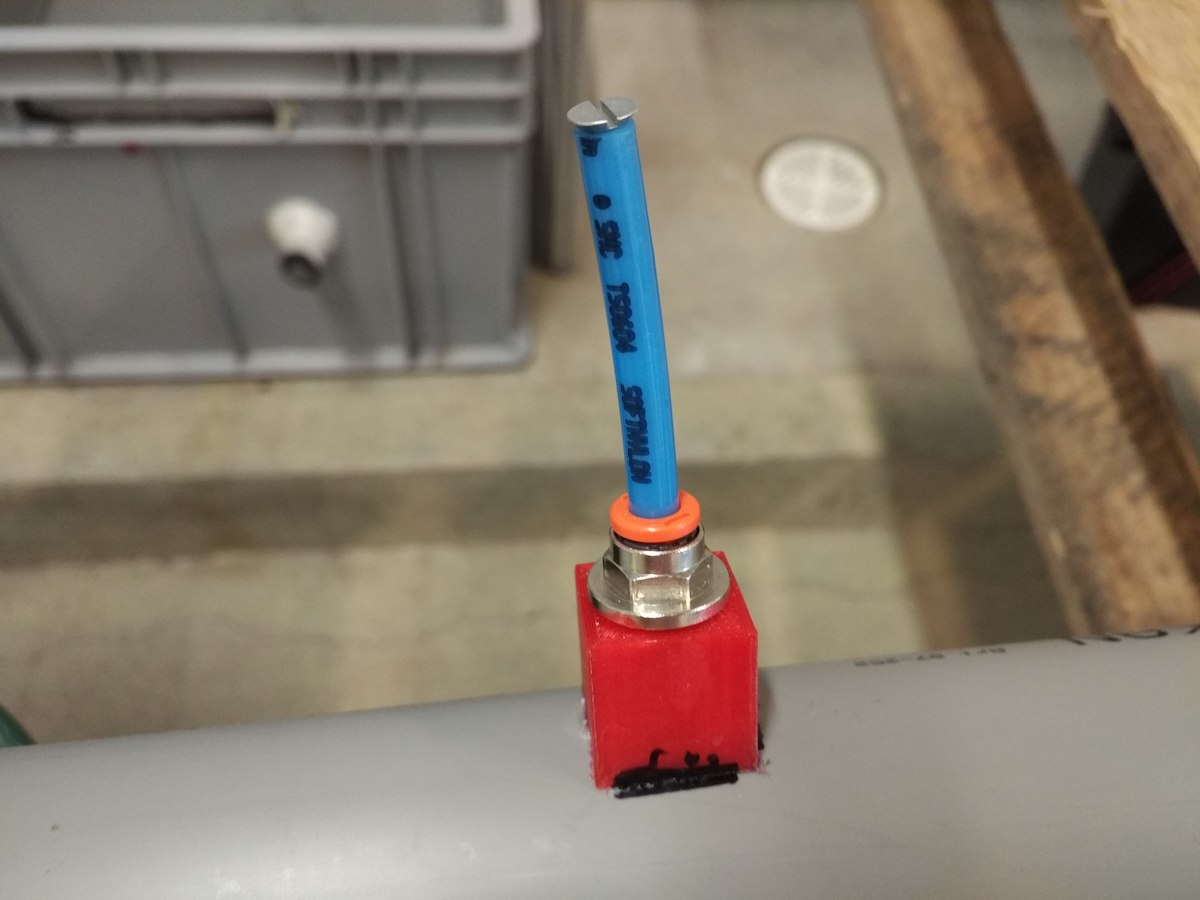
\includegraphics[width=0.9\linewidth]{connector}
     \caption{Connector as measuring points}\label{fig:connector}
   \end{minipage}\hfill
   \begin {minipage}{0.48\textwidth}
     \centering
     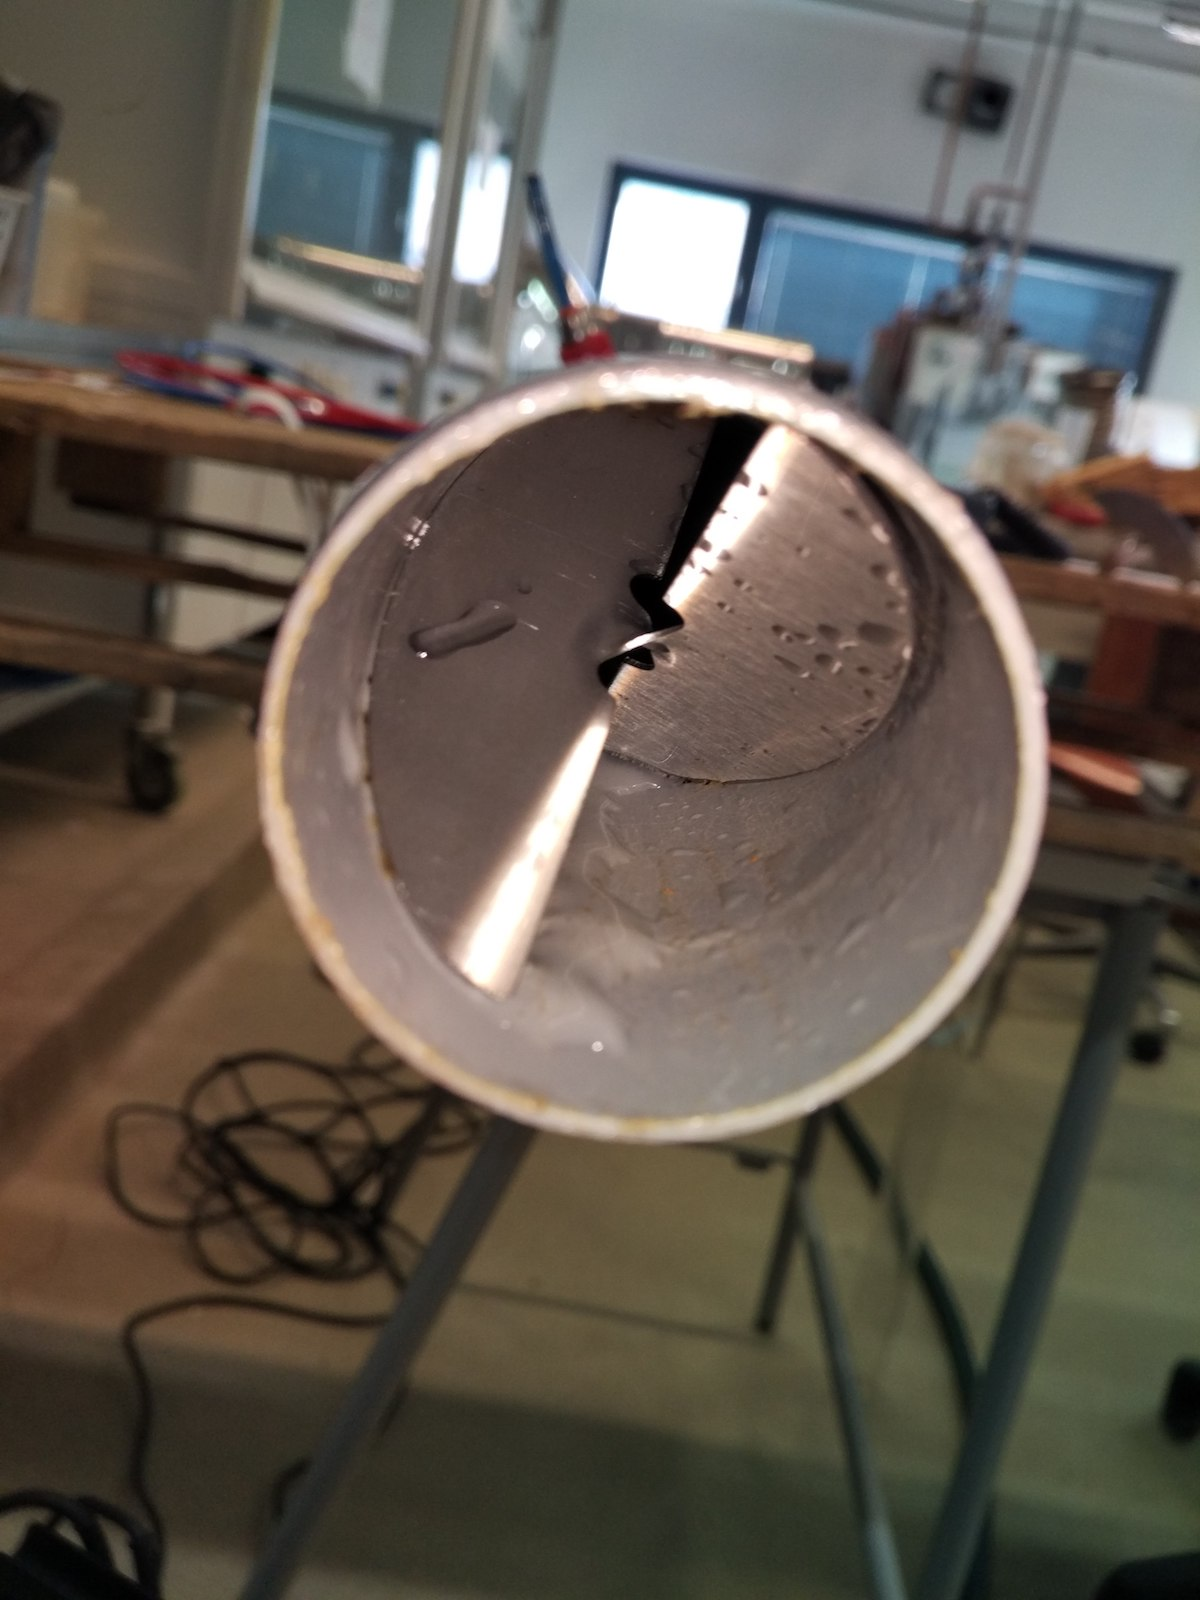
\includegraphics[width=.6\linewidth]{vox}
     \caption{Voxer wing inside pipe}\label{fig:vox}
   \end{minipage}
\end{figure}
\begin{figure}[h]
  \centering
  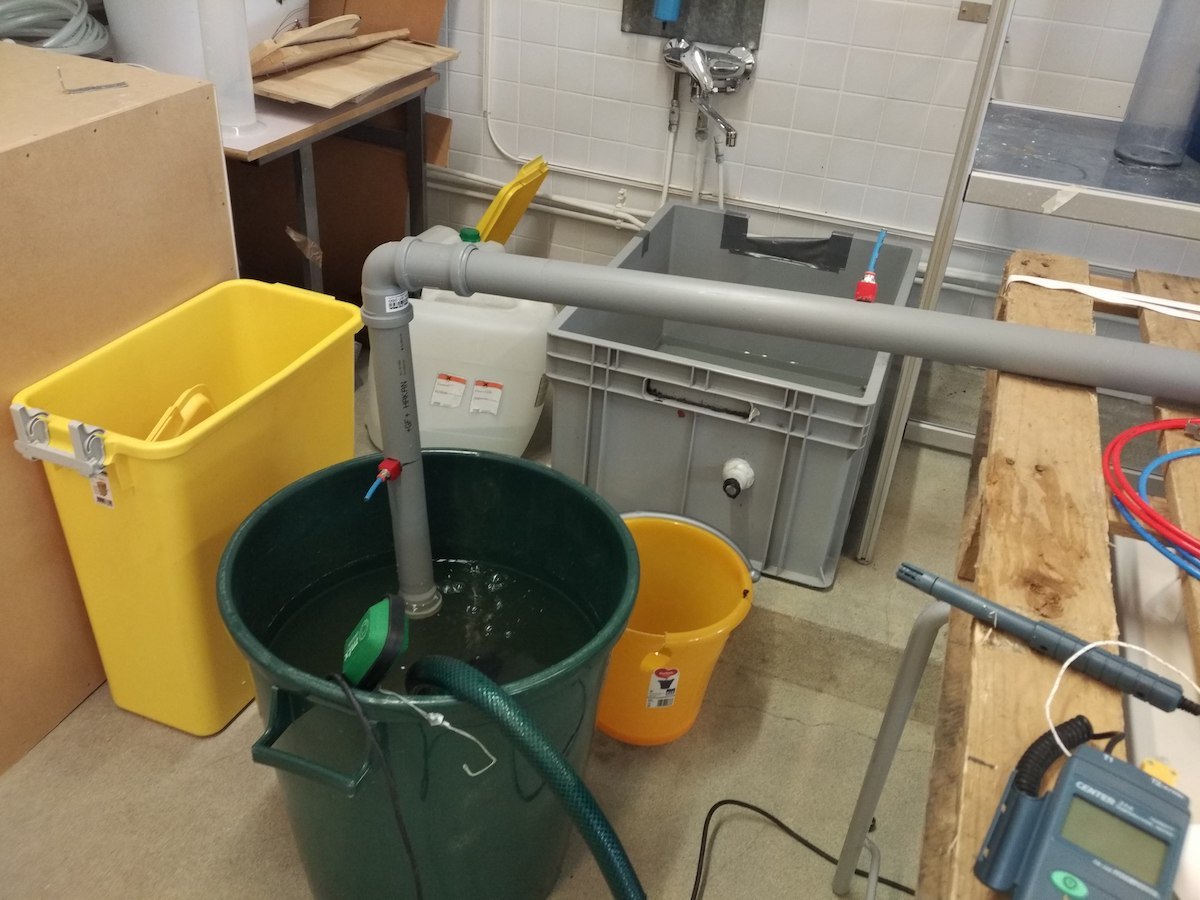
\includegraphics[width=9cm]{sub-pipe}
  \caption{ The ending pipe was submerged into water in reservoir}
  \label{fig:subpipe}
\end{figure}
\subsection{Result and analysis}
Since the data frame acquired from lab experiment is really extensive, the data is treated to take average value of each measurement and demonstrate through the following graphs.
\begin{figure}[h]
  \centering
  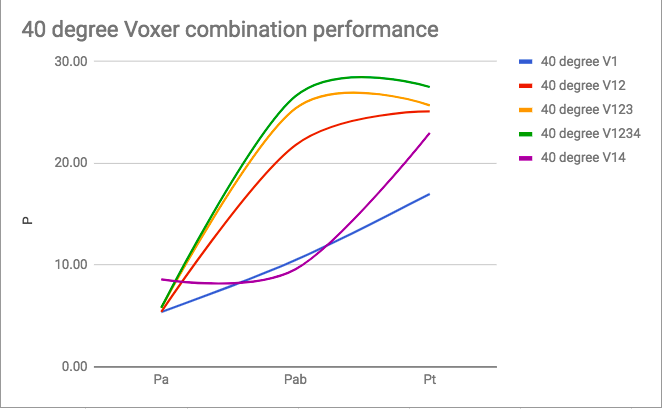
\includegraphics[width=9cm]{40d_graph}
  \caption{ Compare performance of each combination from Voxer 40$^{\circ}$DN40}
  \label{fig:40d}
\end{figure}
In figure \vref{fig:40d}, all of combinations which have Voxer 40$^{\circ}$ DN40 are compared with each other. When the flow started through the 1st Voxer in section A, most of the pressure changes from different combinations result in the similar value around 5 to 7 millibars. Section A has the 1st Voxer before the curve. This show that the behavior of flow after each rotation in pipeline in section A is the same with each other. Starting from section B, we see the drastic change between V1, V14 and the rest of Voxer combinations. The pressure changes between in inflow and before section C are truly dramatic from 7 millibars to more than 25 millibars according to combinations with more than 2 Voxers in pipeline. When comparing pressure of section A and B between combination V1 and V14, V14 is appeared to have less pressure drop than V1. From total pressure drop point of view, V1 has the lowest pressure change while V14 and the rest of combination meet around 24 to 27 millibars. From this graph, it can be seen that 1 Voxer at position V1 results in the lowest pressure change which means that the pressure loss was reduced. 
\begin{figure}[h]
  \centering
  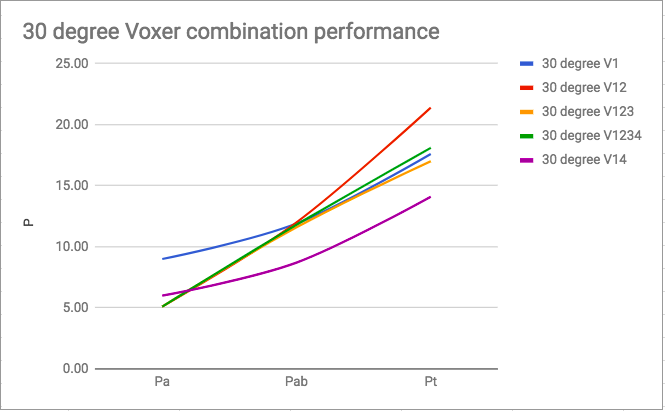
\includegraphics[width=10cm]{30d_graph}
  \caption{Compare performance of each combination from Voxer 30$^{\circ}$ DN40}
  \label{fig:30d}
\end{figure}
Figure \vref{fig:30d} illustrates the operation of Voxer 30$^{\circ}$ DN40 from five Voxer combinations. The trendlines from these combinations of Voxer 30$^{\circ}$ are much more uniform than those trendlines of Voxer 40$^{\circ}$. They all started in section A with a short range of pressure change from 5 to 9 millibars. After section A and B, most of trendlines except V14 meet each other at the intersection of 12 millibars. From here, these trendlines don't separate at total pressure (0.5 to 1 millibar difference) from each other that much except V12 (22 millibars). Meanwhile, V14 keeps the parallel trendlines at the lower level from 6 to 14 millibars.
\begin{figure}[h]
  \centering
  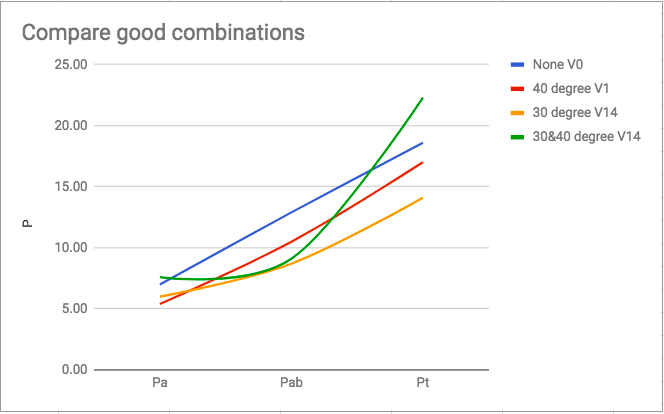
\includegraphics[width=9cm]{compare_graph}
  \caption{ Comparison among good Voxer combinations }
  \label{fig:compare}
\end{figure}
We compare the most potential combination from each Voxer type with the mixed combination and standard pipeline with no Voxer inside in figure \vref{fig:compare}. It can be clearly seen that, the correlation of pressure change along the pipe of standard pipeline, combination V1 of Voxer 40$^{\circ}$ and combination V14 of Voxer 30 $^{\circ}$ DN40 are almost parallel with each other, while the mixed combination V1 (Voxer 30$^{\circ}$) and V4 (Voxer 40$^{\circ}$) leads to the increase in pressure change. Section C is the section with the 4th Voxer placed before the last curve.
\begin{figure}[h]
  \centering
  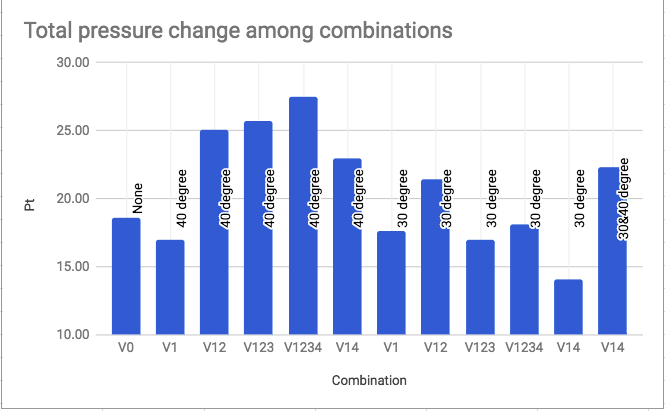
\includegraphics[width=9cm]{Pt_graph}
  \caption{ Total pressure change among all combinations}
  \label{fig:pt}
\end{figure}
From figure \vref{fig:pt}, it can be concluded that the lowest pressure change in total is from combination V14 of Voxer 30$^{\circ}$DN40. Voxer 30$^{\circ}$ performs better than Voxer 40$^{\circ}$. More Voxers in the pipeline, especially inside the main horizontal pipeline would increase pressure change of system in total.  
\section{Experimentation in Keravan Energy}
With the result from the laboratory test, we move on to the design of alternative pipeline in the cooling system. Information about system was given from Keravan Energy. It is known that the income flow rate is around 2 liters per second (local measure) at 1 bar pressure. The input temperature is 6\celsius and the output temperature is 16\celsius. 
Since it is not advised to interfere with the existing pipeline of cooling system, we should assemble an alternative pipeline with characteristics needed for the comparative measurement. In this experiment at Keravan Energy, we observe the behavior of Voxer under realistic uncontrolled condition. The assembly was done in Metropolia's mechanical laboratory.  
\subsection{Experiment's design}
From the observation of original pipeline section (see figure \vref{fig:orgpipe}, it is clear that Voxer couldn't be placed inside rubber hoses but inside straight steel circular pipe. This also applied on positions of measuring points to measure inflow before the curve and outflow after the curve. The water flow rate in Keravan Energy is much higher than the one from pump used in the lab test. So there are chances that water would be leaked from the pipe leading to more energy loss. The fact that Voxer wing should be easy to remove from pipe between different combination is taken into consideration.
\begin{figure}[h]
  \centering
  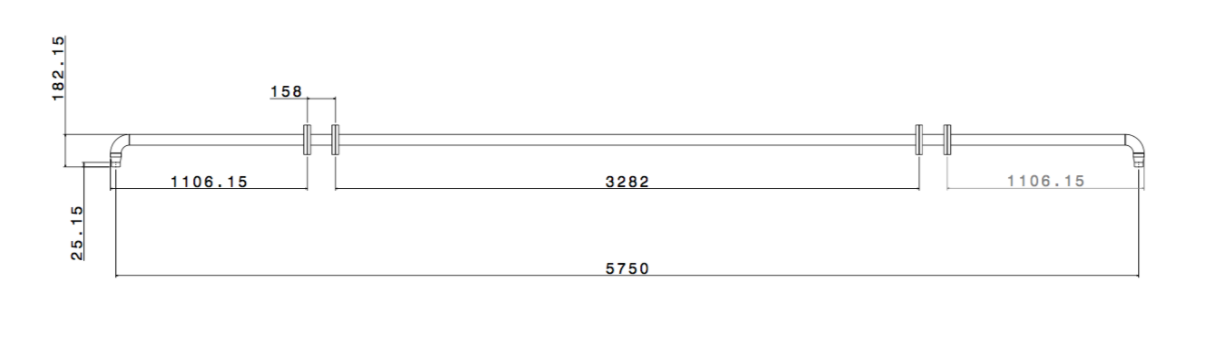
\includegraphics[width=10cm]{cadkerava}
  \caption{ Drawing of pipeline for experiment at Keravan Energy}
  \label{fig:cadkerava}
\end{figure}
A design of pipeline shown in figure \vref{fig:cadkerava} is the experiment's solution for most of problems above. The length of pipeline section was taken from CAD documentation of Keravan Energy and measured again in place. In this setup, there are maximum 2 Voxers tested in the pipeline. Voxer wings were placed from separated pipe (we call them Voxer pipes) with flanges which would easy be connected to the main pipe. 
Rubber hoses were attached to the pipeline by reducers at each side. The measuring points were positioned on the reducers to catch inflow and outflow pressure as well as the middle of long pipe. We divided this testing pipeline into 2 sections. Section A is from inflow reducer to middle point of pipe. Section B is from the middle point to the outflow reducer. The same principles were applied on pressure changes of this pipeline: 
\begin{align}
\delta P_t&= P_ab = P_a + P_b \\
\delta P_ab&= \tn{Total pressure change in pipeline} \\
P_a&= \tn{Pressure change in section A} \\
P_b&= \tn{Pressure change in section B} \\
\end{align}
In this experiment, two types of Voxer were also tested (Voxer $30^{\circ}$ DN50 and Voxer $40^{\circ}$ DN50). The measurements of section B and total pressure were measured by pressure meter. There are three combinations of Voxer in the test: None (indicating empty pipe with no Voxer inside), degree 30 (2 Voxers DN50 $30^{\circ}$), degree 40 ( 2 Voxers DN50 $40^{\circ}$) (see table \ref{table:kerava}). The material of pipes is carbon steel. All of components were purchased from Ahnsell and assembled in Metropolia's mechanical lab.
\begin{table}[h]
  \centering
  \caption{Voxer combinations in Keravan Energy's test}
  \begin{tabular}{l*{2}{c}}
Type             & V0 & V12 \\
\hline
None & X & -   \\
degree 30           & - & X   \\
degree 40          & - & X   \\
\end{tabular}
  \label{table:kerava}
\end{table}
\subsection{Setting of experiments}
\subsubsection{Components Assembly}
\textit{Measuring points}\newline
A metal rod was cut into parts and tapped to create thread for measuring point connectors. Then hole were drilled to create contact space with pressure meter. The cylinder metal parts were welded into reducers and middle point of long pipe above those holes. Figure \vref{fig:coke} presents the final look of measuring points.

\textit{Pipes}\newline
The main 6 meters carbon steel pipe was cut into parts: two Voxer pipes, two side pipes and one long middle pipe. Voxer pipes and long middle pipe were welded with two flanges on each side. Then curves were welded together with side pipes and reducers as a unit. Before welding, the reducers were shaped to fit with rubber hose (see figure \vref{fig:sidepipe}).
\begin{figure}[!htb]
   \begin{minipage}{0.48\textwidth}
     \centering
     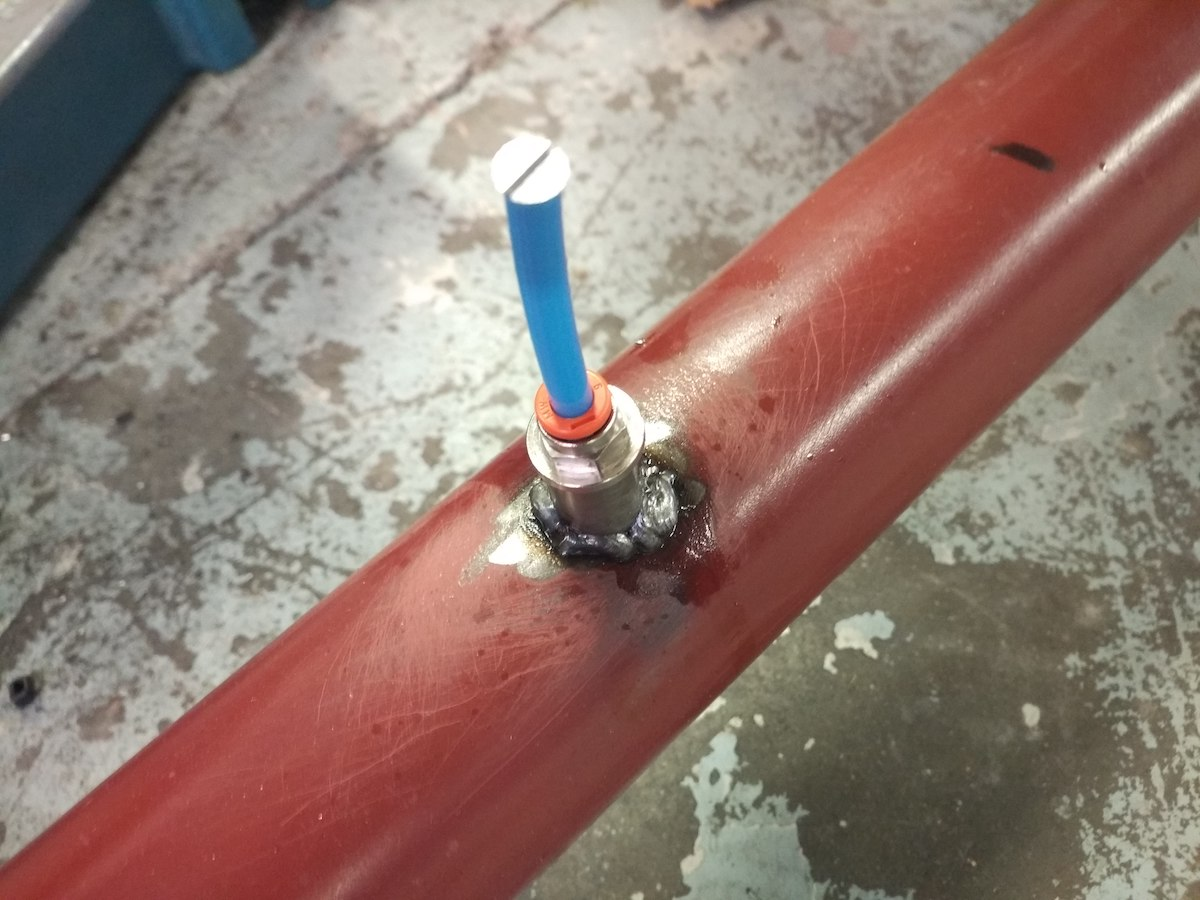
\includegraphics[width=0.7\linewidth]{connect_ke}
     \caption{Metal connector as measuring points}\label{fig:coke}
   \end{minipage}\hfill
   \begin {minipage}{0.48\textwidth}
     \centering
     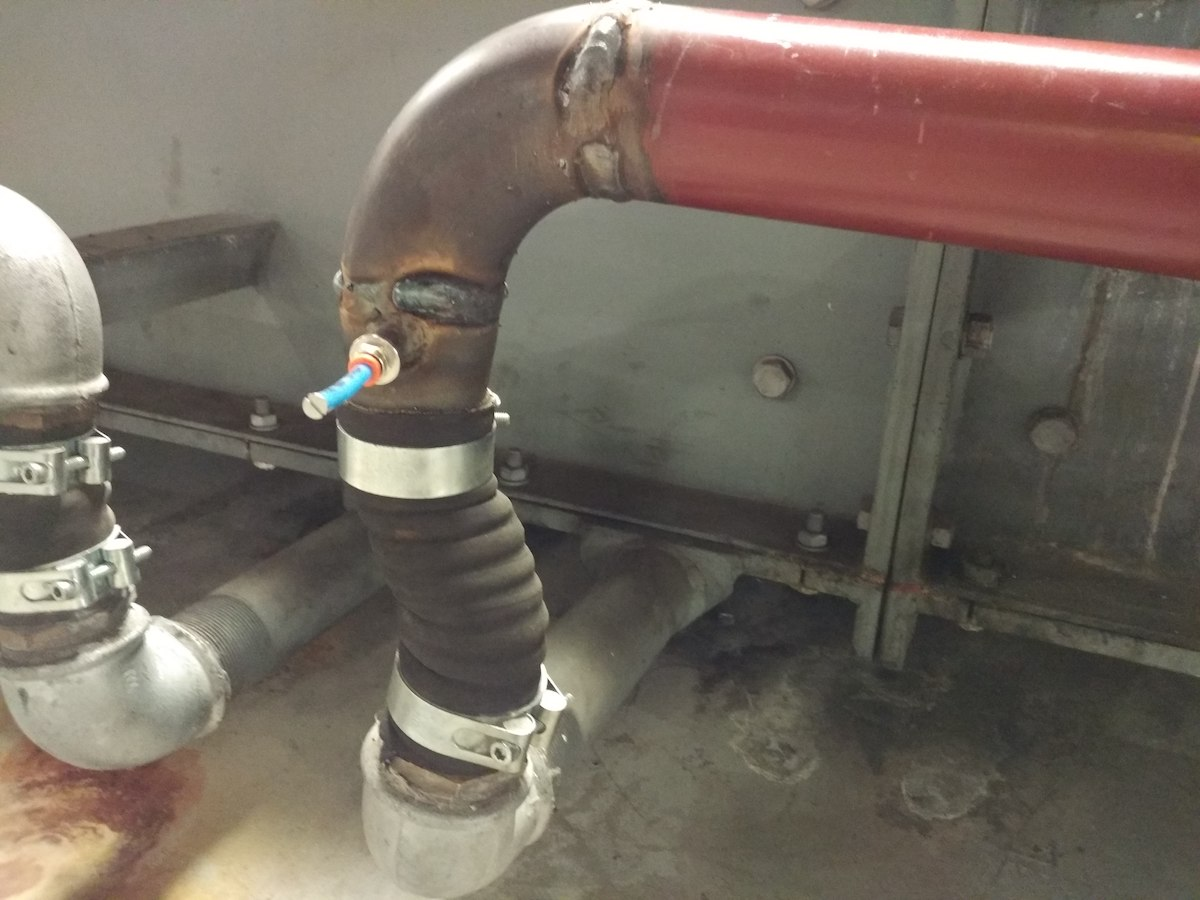
\includegraphics[width=.7\linewidth]{new_side_pipe}
     \caption{Curve, reducer and side pipe}\label{fig:sidepipe}
   \end{minipage}
\end{figure}
\subsubsection{Setting up in Keravan Energy}
At Keravan Energy, the original pipeline section was removed and altered with our testing pipeline. The frame was raised to hold the weight of the new pipeline with higher height than the original one. New rubber hoses were cut to fit the new pipeline. After testing and adjusting some minor problems in the system, the flow rate was adjusted from 2 to 0.8 liters per second to reduce pressure applied on minor leaking points along the pipe. Figure shows an overview of the setting.
\begin{figure}[h]
  \centering
  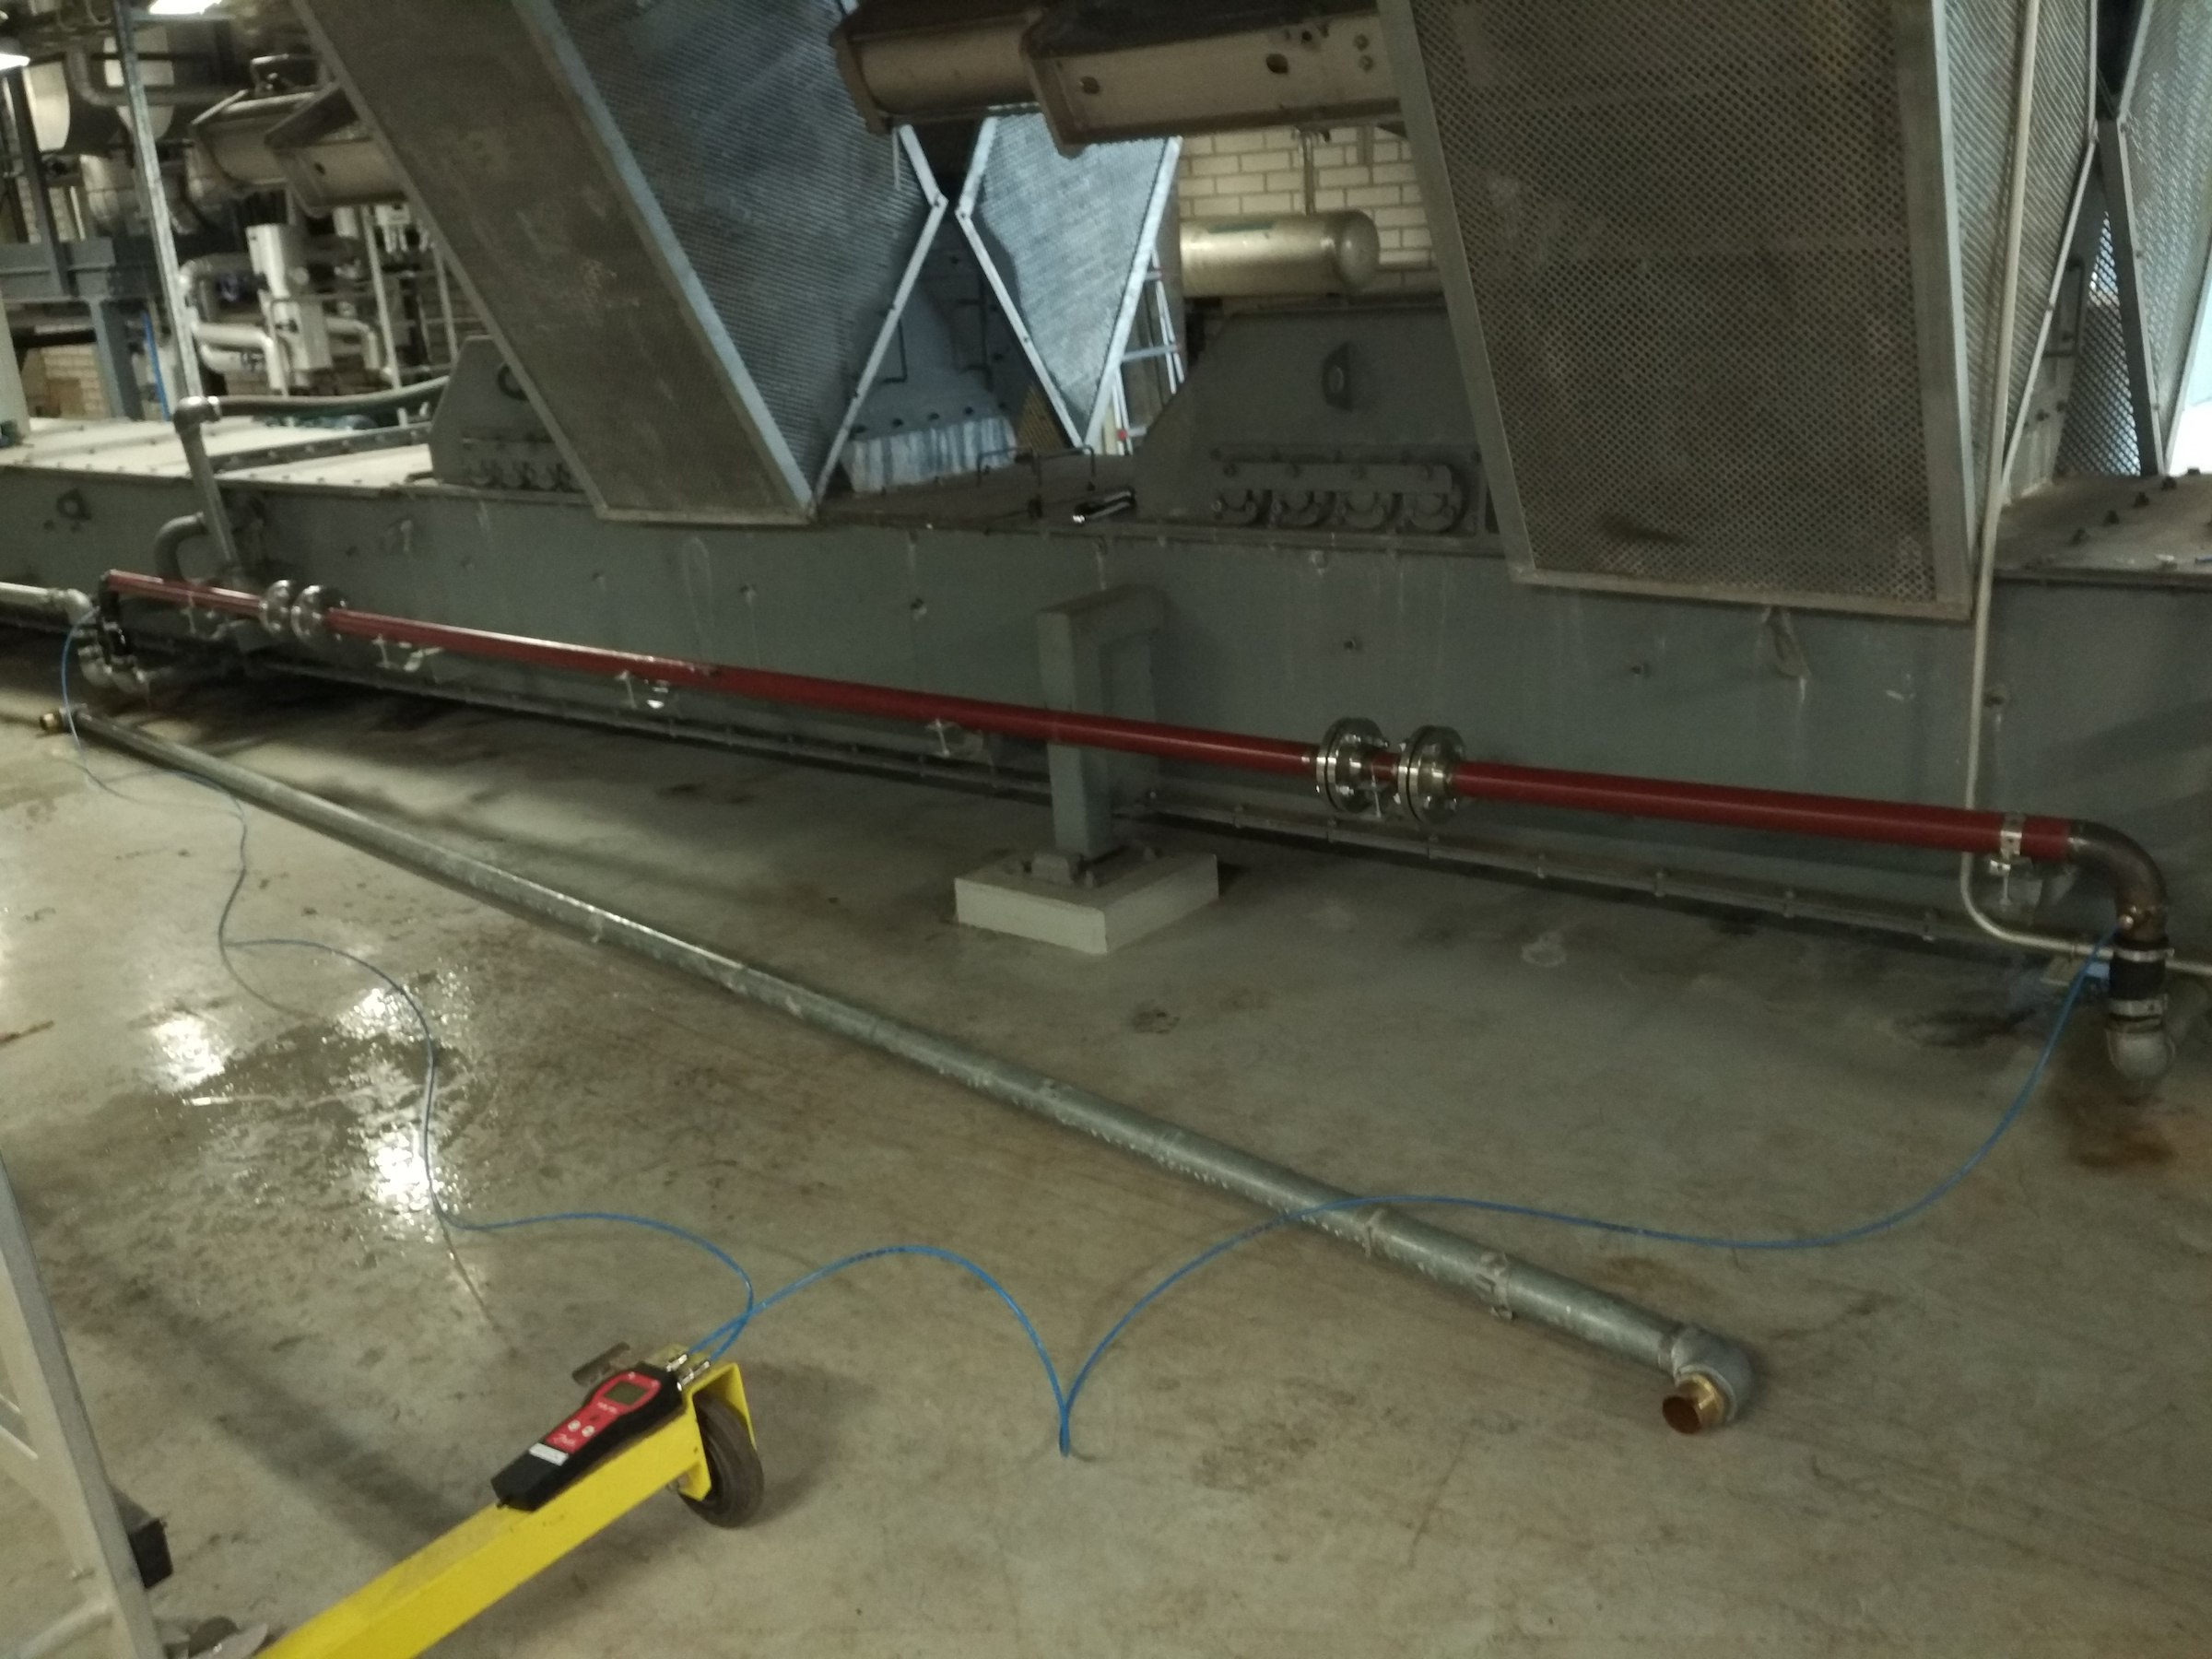
\includegraphics[width=9cm]{overview_test}
  \caption{ An overview of the testing pipeline}
  \label{fig:overview}
\end{figure}
\subsection{Result and analysis}
From the observations through the pressure meter, the pressure values of each measurement were not stable and varying in a large range. The result from Kervan Energy experiment was not as accurate as the result from lab experiment since the measurement was performed under uncontrolled condition in such limited amount of time. Therefore each measurement was recorded and transcribed into separate CSV files. In the experiment, P$_{\text{b}}$ and P$_{\text{ab}}$ were recorded. There are 100 points from each measurement transcribed. The flow rate of the system was maintained around 0.8 liters per second throughout the whole experiment. There were some minor water leaking around measuring points as well.

From Figure a, it can be seen that the total pressure inside the empty piping section varies in a large range from -10 to 30 millibars. The negative values can be explained as the possibility of cavitation occurrence due to high velocity. The most occurring pressure values are ranged from 10 to 20 millibars. The dotted line illustrated smoothened density line of total pressure in empty pipe. 

It is illustrated in figure , the total pressure of a combination of two Voxers 30$^{/circ}$. Values ranges vastly from 0 to 50 millibars. The most popular values in this combination varies from 20 to 40 millibars.

There are some differences in combination Voxer 40$^{/circ}$ with empty pipe and Voxer 30$^{/circ}$. The distribution of 2 other graphs show the pattern of normal distribution while this graph shows large range of value distribution. Values vary from 40 to 90 millibars, which is much higher than measurements from empty pipe and Voxer 30$^{/circ}$. Pressure change values occur most around 50 to 65 millibars and from 75 to 80 millibars. 

Each point in figure represents pressure value of section B with 2nd Voxer in the piping section throughout recorded times. The line smoothens the trend of pressure values in each type of combination. From here, we can see that .


\clearpage %force the next chapter to start on a new page. Keep that as the last line of your chapter!

%% Conclusions

\chapter{Conclusions}

Check Final Year Project Guide for the content of Conclusions chapter.

\clearpage %force the next chapter to start on a new page. Keep that as the last line of your chapter!


% Sample content to demonstrate LaTeX command. You will likely delete this line and the 
% next \input{sample/*} lines. You are also safe to delete the sample/ folder and its
% content once you refershed your LaTeX skills. Also check the appendix samples.
\input{sample/1content.tex}
\input{sample/2lorem.tex}
\input{sample/3graph.tex}

%----------------------------------------------------------------------------------------
%	BIBLIOGRAPHY REFERENCES
%----------------------------------------------------------------------------------------

\input{style/biblio.tex}

%----------------------------------------------------------------------------------------
%	APPENDICES 
%----------------------------------------------------------------------------------------

\input{style/appendix.tex}
%force smaller vertical spacing in table of content
%!!! There can be some fun depending if the appendices have (sub)sections or not :D
% You will have to play with these numbers and eventually add the \vspace line  before 
% some \chapter and force another number.
% To add more fun, time to time the table of content get wrong after a build :(
\addtocontents{toc}{\vspace{11pt}}
\pretocmd{\chapter}{\addtocontents{toc}{\protect\vspace{-24pt}}}{}{}

\liite{1}% This is a hack to have right page numbering for each appendix. Make sure to 
	 % use a unique number for each appendix.
% Appendix 
% And demonstrate text references and bibliography references in appendix

\chapter{Data analysis}\label{appx:first}

\section{Mean value of data from laboratory experiment}

\begin{table}[h!]
\centering
\begin{tabular}{ | l | l | l | l | l |  }
\hline
Type & Delta P  & $P_{a}$ & $P_{b}$ & $P_{t}$ \\
\hline
None & V0 & 7.00 & 12.90 & 18.60 \\ \hline
\multirow{5}{*}{40$^{\circ}$} & V1 & 5.40 & 10.50 & 17.00 \\
 & V12 & 5.40 & 21.80 & 25.10 \\
 & V123 & 5.80 & 25.40 & 25.70 \\
 & V1234 & 5.80 & 26.60 & 27.50 \\
 & V14 & 8.60 & 9.60 & 23.00\\ \hline
\multirow{5}{*}{30$^{\circ}$} & V1 & 9.00 & 11.90 & 17.60 \\
 & V12 & 5.10 & 12.00 & 21.40 \\
 & V123 & 5.10 & 11.60 & 17.00 \\
 & V1234 & 5.10 & 11.80 & 18.10 \\
 & V14 & 6.00 & 8.70 & 14.10\\ \hline
30$^{\circ}$- 40$^{\circ}$ & V14 & 7.60 & 9.10 & 22.30 \\ \hline
\end{tabular}
\end{table}

\section{R code for analysis of Keravan experiment}
\begin{code}
  \inputminted{r}{code/test.R}
  \captionof{listing}{R code}
  \label{code:rcode}
\end{code}

\clearpage %force the next chapter/appendix to start on a new page. Keep that as the last line of your appendix!

% Sample content to demonstrate appendix in LaTeX. You
% are safe to delete this lines (and the next samples) once you refreshed your LaTeX 
% skills (and safe to delete the sample folder and all its file too).

\addtocontents{toc}{\vspace{11pt}}%fix vertical space for Table of Content
\liite{2}
\input{sample/Xappendix2.tex}

\addtocontents{toc}{\vspace{11pt}}
\liite{3}
\input{sample/X_R_example.tex}


%----------------------------------------------------------------------------------------
%	THIS IS THE END 
%----------------------------------------------------------------------------------------
\end{document}
